\documentclass[conference]{IEEEtran}
\usepackage[utf8]{inputenc}
\usepackage[T1]{fontenc}
\usepackage{amsmath,amssymb}
\usepackage{graphicx}
\usepackage{booktabs}
\usepackage{multirow}
\usepackage{hyperref}
\usepackage{enumitem}
\usepackage{balance}
\usepackage{cite}
\usepackage{url}
\usepackage{tikz}
\usetikzlibrary{arrows.meta,positioning}

\title{Policy-Grounded Agentic Control for Safe Purchase-to-Pay Automation}

\author{\IEEEauthorblockN{Rayyan Azmat}
\IEEEauthorblockA{Department of Computer Science\\
AI4015 Semester Project\\
Roll No.: P220507\\
\href{mailto:rayyanazmat722@gmail.com}{rayyanazmat722@gmail.com}}}

\begin{document}
\sloppy
\maketitle

\begin{abstract}
Purchase-to-pay (P2P) automation is a safety-critical operational domain in which incorrect clearance can create financial, compliance, and audit risk. We study a policy-instrumented workflow in a deterministic local simulator, combining explicit risk checks, an approval controller, and server-side state-transition guards. In a 100-case synthetic evaluation, the policy-enabled ReAct configuration reached exact match 1.00, reported risk alerts for 0.40 of cases, and recorded no unsafe mutation; its intervention rate was 0.40. With policy detection disabled, exact match and intervention remained unchanged while the alert metric fell to zero because the detector was off. An eight-configuration ablation reproduced this pattern; approval toggling did not change aggregate metrics. A 100-case BPI Challenge 2019 replay also reached 1.00 agreement with reconstructed proxy labels, which are not invoice-level ground truth. These deterministic, offline results show that policy instrumentation changes recorded risk visibility in the fixture, but do not establish improved real-world safety, causal benefit, or LLM reasoning performance.
\end{abstract}

\begin{IEEEkeywords}
Purchase-to-pay, agentic AI, workflow governance, safety, invoice verification, human-in-the-loop automation.
\end{IEEEkeywords}

\section{Introduction}

Agentic systems are increasingly used to automate operational workflows in enterprise settings; however, in domains such as procurement, financial controls, and audit-sensitive processing, a superficially plausible action can still be unsafe in practice. The key challenge is not only whether a system reaches a valid terminal state, but also whether it avoids policy-breaking transitions, exposes contradictory evidence, and supports human review when the evidence is incomplete or risky. This is especially important in purchase-to-pay (P2P) workflows, where an invoice can be cleared too early, a receipt may be incomplete, or duplicate evidence may be ignored.

This paper studies the following question: how do explicit policy checks and review controls affect end-state correctness, policy-risk visibility, and execution cost in a P2P workflow? Three gaps motivate the evaluation. First, tool-using workflows need explicit controls around multi-step state changes. Second, results from formal or synthetic process studies need to be tested against procurement traces, while distinguishing observed event data from reconstructed transaction labels. Third, correctness alone does not capture review burden, risk visibility, or execution cost.

We implement a deterministic local simulator, an explicit policy engine, an approval controller, and compensation safeguards. The experiments compare an ungated ReAct configuration with the policy- and approval-enabled configuration, a deterministic heuristic comparator, a BPI Challenge 2019 trace-derived replay, and a factorial ablation. The BPI replay is reported only as a proxy-label transfer test: the source event log does not contain invoice-level ground truth.

The contributions are (1) a locally reproducible P2P simulator and fixed synthetic manifest; (2) policy, review, and recovery modules whose state is observable through tool traces; and (3) a comparative evaluation reporting end-state match, policy-risk alerts, unsafe mutations, interventions, latency, token estimates, and tool calls. The experiments do not establish that the governance components improve terminal accuracy: all variants attain 1.00 match on this deterministic fixture, and the simulator independently blocks invalid mutations. The narrower empirical result is that policy checks surface risky input cases without reducing measured correctness.

\section{Related Work}

Process mining represents and analyzes recorded behavior through event logs, while business-process management supplies modeling and lifecycle concepts for organizing that behavior \cite{aalst2012manifesto,aalst2016process,aalst2004workflow,dumas2018fundamentals,mendling2010guidelines}. Declarative workflow models are relevant when a process has constraints but permits multiple valid execution paths. Pesic and van der Aalst formalize a declarative approach, and subsequent work studies the balance between flexibility and execution support \cite{pesic2006declarative,aalst2009declarative}. These foundations motivate explicit workflow conditions in the P2P simulator, but our implementation is a rule-based control layer rather than a Declare translation system.

The selected base paper by Fionda et al. studies whether language models can translate Declare constraints through natural language while preserving semantic properties. Its symbolic checking approach is adjacent to, but not the same task as, executing purchase-to-pay transactions \cite{fionda2025large}. Recent process-oriented work studies rule-grounded agents, process knowledge acquisition, process modeling, workflow generation, simulation, and process-mining benchmarks \cite{kaltenpoth2025rules,schinckus2026process,qiao2025benchmark,jha2025itbench,kirchdorfer2025multiagent,dasilva2025declarative,kourani2026modeling,rebmann2025semantics,berti2025pmllm}. This literature indicates that process structure and evaluation design matter, but the datasets, metrics, and tasks differ. In particular, we do not claim to reproduce Fionda et al.'s Declare translation procedure; our heuristic comparator is not a base-paper reproduction.

Tool-using language-model research includes interleaved reasoning and actions, learned tool selection, multi-agent orchestration, and agent evaluation in interactive environments \cite{yao2023react,schick2023toolformer,wu2023autogen,qin2024toolllm,liu2024agentbench,zhou2024webarena,brown2020fewshot,openai2023gpt4}. These systems make it important to distinguish a planner's proposed action from an environment's accepted state transition. Our simulator records both. In human factors research, automation can be misused, underused, or over-trusted; models of human interaction and practical human-AI guidelines emphasize calibrated control and understandable intervention \cite{parasuraman1997automation,parasuraman2000interaction,amershi2019guidelines,nist2023airmf}. Here, the review layer is a deterministic approval rule, not a user study; no claim about human reviewer effectiveness is made.

\section{Problem Formulation}

Let a case $c$ be represented by a purchase-order state $PO$, an invoice state $INV$, and a receipt state $GR$. The agent must choose an action from the constrained set $\mathcal{A} = \{\text{clear}, \text{hold}, \text{verify\_receipts}, \text{escalate}\}$. A transition is valid only if the evidence is internally consistent and complies with the rule set encoded in the policy layer.

The system monitors several important failure modes. These include duplicate or contradictory evidence, invoice-to-PO amount mismatch, incomplete receipt quantities, missing verification before final clearance, and unsafe post-hoc clearance after a warning or hold. Formally, the objective is not simply to maximize clearance rate, but to maximize safe, audit-ready transitions while minimizing policy violations and uncontrolled automation.

The goal is therefore a constrained decision problem: choose actions that preserve end-state correctness while maintaining explicit checks on evidence quality and policy compliance. This distinction is crucial because high throughput and high correctness are not equivalent to safe operation in procurement contexts.

For experimental reporting, the state of a case at step \(t\) is represented as \(s_t=(p_t,i_t,g_t,h_t,a_t)\): purchase-order evidence, invoice state, goods-receipt evidence, hold/review state, and audit history. An agent proposes \(a_t\in\mathcal{A}\), and the simulator applies a transition function \(T(s_t,a_t)\) only when its server-side preconditions pass. The policy evaluator separately maps the observed state to a set \(r(s_t)\) of risk rules. This yields three non-equivalent outcomes: a risk report \(r(s_t)\ne\emptyset\), a rejected mutation where \(T\) does not apply, or an applied mutation that ends in an unexpected terminal state. This paper measures each separately rather than collapsing them into a single "failure" label.

We do not combine the measures into a weighted utility function because no stakeholder-approved trade-off weights are available. Instead, we report a metric vector \((\mathrm{EM}, \mathrm{alert}, \mathrm{unsafe}, \mathrm{intervention}, \mathrm{latency}, \mathrm{calls}, \mathrm{tokens})\) for each configuration. This preserves the distinction between transaction outcome, detection behavior, oversight signal, and computational effort. In particular, a higher alert or intervention rate is not inherently better: its interpretation depends on the risk prevalence and the quality and cost of subsequent human review, neither of which is estimated from these simulator experiments.

\section{System Architecture and Methodology}

The evaluated workflow separates state observation, decision logic, and environment enforcement. This separation is important for interpreting results: a policy alert describes a risky case; a rejected tool call describes an attempted action that violated a server invariant; and an unsafe mutation would be a completed transition to an invalid state. These are different events and are reported separately.

\begin{figure}[t]
\centering
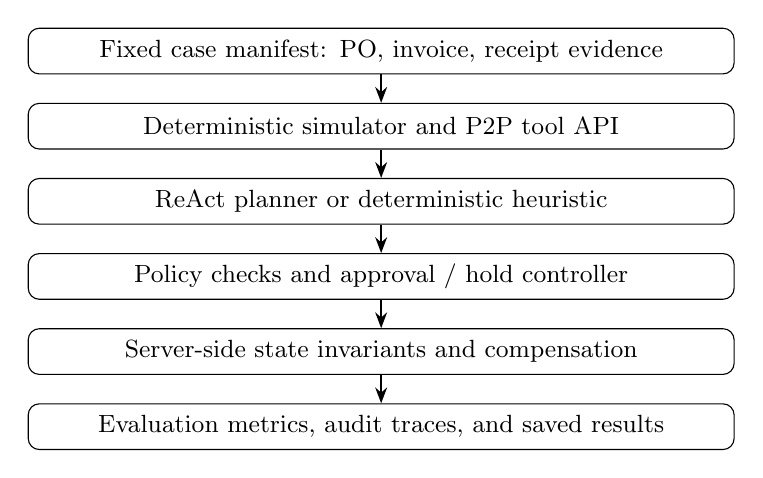
\begin{tikzpicture}[
  node distance=0.36cm,
  block/.style={draw, rounded corners, align=center, text width=0.72\columnwidth, minimum height=0.58cm, font=\small},
  arrow/.style={-{Stealth[length=2mm]}, thick}
]
\node[block] (data) {Fixed case manifest: PO, invoice, receipt evidence};
\node[block, below=of data] (sim) {Deterministic simulator and P2P tool API};
\node[block, below=of sim] (agent) {ReAct planner or deterministic heuristic};
\node[block, below=of agent] (policy) {Policy checks and approval / hold controller};
\node[block, below=of policy] (guard) {Server-side state invariants and compensation};
\node[block, below=of guard] (eval) {Evaluation metrics, audit traces, and saved results};
\draw[arrow] (data) -- (sim);
\draw[arrow] (sim) -- (agent);
\draw[arrow] (agent) -- (policy);
\draw[arrow] (policy) -- (guard);
\draw[arrow] (guard) -- (eval);
\end{tikzpicture}
\caption{Local deterministic P2P workflow evaluated in this study. The simulator remains the final authority on accepted state transitions.}
\label{fig:architecture}
\end{figure}

\subsection{Deterministic benchmark environment}

The project uses a local simulator rather than a production ERP connection. Each case contains a purchase-order item, invoice, expected terminal invoice status, matching category, invoice verification flag, duplicate-invoice flag, and receipt events. The simulator exposes reads for purchase orders, invoices, receipts, and audit history, as well as mutations for receipt verification, invoice clearance, and case holds. A reset endpoint seeds a run from a frozen manifest so that each configuration receives the same initial state.

The primary synthetic manifest contains 100 cases with seed 2019. It includes 20 cases each for two-way matching, complete three-way matching, three-way matching with missing goods receipt, consignment, and a fault-injected category. The expected terminal statuses are 60 cleared and 40 held. Fault labels include five amount mismatches, five duplicate invoices, five incomplete receipts, and five unverified invoices; 80 records have no injected fault. These counts describe the constructed fixture, not the prevalence of faults in operational procurement systems.

\begin{table}[t]
\centering
\caption{Composition of the synthetic evaluation manifest.}
\label{tab:manifest}
\begin{tabular}{lrr}
\toprule
Scenario stratum & Cases & Expected status \\
\midrule
Two-way match & 20 & Cleared \\
Complete three-way match & 20 & Cleared \\
Consignment & 20 & Cleared \\
Three-way, missing receipt & 20 & Held \\
Fault-injected evidence & 20 & Held \\
\midrule
Total & 100 & 60 cleared / 40 held \\
\bottomrule
\end{tabular}
\end{table}

The transfer test uses a separate 100-case manifest derived from the BPI Challenge 2019 event log, whose source record is the 4TU.ResearchData dataset \cite{vandongen2019bpi}. The source is event-log data grouped by purchase-order document; it does not contain invoice identifiers, invoice-level amounts, item quantities, or definitive hold decisions. The replay builder reconstructs such fields and conservative expected statuses. Consequently, the BPI test measures behavior on trace-derived scenarios against proxy labels, not accuracy against observed invoice outcomes.

\subsection{Policy engine}

The policy layer inspects each case before a final decision is taken. It checks invoice verification, duplicate evidence, amount mismatches, and incomplete receipt quantities. These checks are represented explicitly in code and are therefore auditable. In practice, this means the system does not simply rely on the agent to infer whether an action is safe; it also applies rule-based constraints before the final state transition can occur.

For a case \(c\), let \(r(c)\) be the set of policy rules violated by its input evidence. The policy layer emits an alert when \(r(c)\neq\emptyset\). The action controller may then request verification or hold the case; the simulator independently validates each state-changing request. The present code's reported policy-violation metric is operationally a *policy-risk alert rate*: it counts cases with a policy report or a relevant rejected tool request. It does not mean that an unsafe transaction was completed. This distinction is especially important in the policy-off ablation, where the alerting component is disabled and therefore cannot be interpreted as a zero underlying-risk rate.

\subsection{Approval and intervention logic}

The orchestration layer decides whether a case should be held, reviewed, or escalated. This is essential in ambiguous cases where the evidence is partial or contradictory. The controller converts policy violations into operational interventions rather than silently allowing the workflow to continue. In this way, the system makes the intervention rate a measurable quantity instead of an implicit side effect.

The approval controller assigns fixed risk weights: 35 points for an unverified invoice, 55 for duplicate evidence, 40 for an amount mismatch, and 35 for incomplete quantity under three-way or consignment matching. An already-held invoice adds 20 points; the total is capped at 100. Expected terminal labels are withheld from controller inputs and used only by the evaluator after execution. If no policy rule is violated and the score is below 30, the controller recommends approval. A score of at least 60 or a critical policy result recommends a hold; a remaining policy violation recommends review. These thresholds are implementation constants, not empirically calibrated probabilities, and the score should not be interpreted as a statistical risk estimate.

The execution sequence in each evaluation run is therefore: (1) reset the simulator from the selected manifest; (2) read the purchase order, invoice, and receipt evidence; (3) evaluate policy and approval settings; (4) issue a clear, verify, hold, or review-related action; and (5) read back the terminal state and audit trace for metric calculation. The environment records rejected actions as tool-call outcomes and does not apply the corresponding state transition. The fixed, offline ReAct backend produces structured actions; it does not generate free-form reasoning with a hosted foundation model. This makes the evaluation repeatable while leaving natural-language model behavior outside the scope of the present evidence.

\subsection{Safeguard and compensation layer}

When a risky state is detected, the safeguard layer applies a compensating action or a controlled hold. This prevents a bad state from propagating silently through later actions. In the benchmark, representative cases such as SYN-041 and SYN-081 are held because receipt quantity is incomplete or evidence is inconsistent, while SYN-021 and SYN-061 are only cleared after the system verifies receipt completeness and consistency.

The simulator also checks transition preconditions on the server side. In particular, an invoice cannot be cleared when required checks fail. Compensation plans are represented as explicit suggested actions for missing verification, duplicate evidence, amount mismatch, incomplete receipt, or an unexpected cleared state. The measured unsafe-mutation rate is the fraction of cases that actually end in a cleared state although their expected state is held. A zero value therefore reports no observed incorrect clearance in this fixture; it does not prove that compensation logic would work against an external ERP.

\subsection{Decision and enforcement boundaries}

The workflow has three control points. First, the agent reads the case state and proposes an action. Second, policy evaluation determines whether the observed fields match configured risk rules and whether the action should be held or escalated. Third, the simulator validates the requested state change against independent invariants and records accepted transitions in the audit history. Keeping these points distinct allows the evaluation to report what was detected, what was requested, and what state change actually occurred.

This design also sets a limit on the causal conclusions available from the experiment. Disabling the policy layer does not remove the simulator's state-transition invariants, and disabling approval does not alter the case manifest or the acceptance rules of the simulator. The off conditions are therefore not equivalent to an unguarded payment environment. An experiment that removed both controller checks and server invariants would require a separately isolated sandbox, because permitting unsafe state changes in a live payment system would be unacceptable. The current benchmark prioritizes safe local testing over that stronger causal intervention.

\subsection{Evaluation metrics}

Let \(N\) denote the number of cases. For case \(i\), let \(y_i\) be the expected terminal status and \(\hat y_i\) the observed status. Exact match is
\[
\mathrm{EM}=\frac{1}{N}\sum_{i=1}^{N}\mathbb{1}[\hat y_i=y_i].
\]
Policy-risk alert rate is the fraction of cases on which the enabled policy layer reports a risk condition. It is not a completed-violation rate: an alerted case can correctly terminate in a hold. Unsafe-mutation rate is the fraction of cases whose final state is an invalid clearance when a hold is expected. Intervention rate is the fraction of cases marked for hold or review. When policy detection is off, the alert field is mechanically zero and is not evidence that the underlying cases have no risk. Latency is elapsed local wall-clock time per case; p95 is the empirical 95th percentile. Tool calls per case are the mean number of logged simulator calls. Token counts are estimates from the offline scripted backend, not tokenizer-verified hosted-model usage.

The measurements are descriptive statistics for fixed deterministic manifests and one recorded run per configuration. We do not report inferential tests or confidence intervals because the benchmark does not sample independent operational transactions, and the measurements are not repeated stochastic model trials.

\section{Evaluation Methodology}

The evaluation uses a frozen synthetic manifest of 100 cases (seed 2019) and a 100-case BPI-derived replay. The full evaluation driver records E1--E4 and E6 outputs; the factorial study is run separately. The repository stores per-experiment JSON, aggregate summaries, and representative case traces. The primary reproduction commands, executed from the project directory, are:

\footnotesize
\begin{verbatim}
python experiments/run_evaluation.py
python main.py --ablation-study \
  --cases 100
\end{verbatim}
\normalsize

The representative trace exporter is \path{experiments/export_representative_traces.py}.

E1 is the ReAct baseline with policy and approval disabled. E2 is an explicitly identified deterministic heuristic comparator with controls on; it is not a reproduction of the Phase 1 base paper, which addresses natural-language translation of Declare constraints. E3 enables the policy and approval controls with ReAct. E4 replays BPI-derived cases using the ReAct and heuristic configurations. E5 independently toggles policy and approval for each agent, producing eight 100-case configurations. E6 compares local efficiency measurements for the two agents with controls on. All runs use an offline scripted agent backend and local simulator; they do not call a hosted LLM or an ERP.

The benchmark therefore evaluates whether the control pipeline makes its decisions observable and preserves the fixture's expected outcomes, not whether an LLM generalizes to unseen invoices. The deterministic data, offline agent, and server-side transition checks constrain what can be inferred: the experiments can compare recorded behaviors under controlled toggles, but cannot estimate performance under production variation.

\section{Results}

\begin{table*}[t]
\centering
\scriptsize
\setlength{\tabcolsep}{3pt}
\caption{E1--E4 benchmark results. Policy-risk alerts are detector outputs; E1 has no detector enabled. BPI-derived labels are proxies rather than invoice ground truth.}
\label{tab:benchmark}
\begin{tabular}{lp{0.21\textwidth}rrrrrrr}
\toprule
Experiment & Configuration / data & \(N\) & Exact match & Risk alert & Unsafe mutation & Intervention & p95 (s) & Calls/case \\
\midrule
E1 & ReAct, controls off; synthetic & 100 & 1.00 & 0.00\(^a\) & 0.00 & 0.40 & 0.0137 & 6.20 \\
E2 & Heuristic, controls on; synthetic & 100 & 1.00 & 0.40 & 0.00 & 0.40 & 0.0112 & 5.40 \\
E3 & ReAct, controls on; synthetic & 100 & 1.00 & 0.40 & 0.00 & 0.40 & 0.0114 & 6.20 \\
E4 & ReAct, controls on; BPI proxy & 100 & 1.00\(^b\) & 0.55 & 0.00\(^b\) & 0.55 & 0.0111 & 6.17 \\
E4-H & Heuristic, controls on; BPI proxy & 100 & 1.00\(^b\) & 0.55 & 0.00\(^b\) & 0.55 & 0.0085 & 5.39 \\
\bottomrule
\end{tabular}
\vspace{1mm}
\begin{minipage}{0.96\textwidth}
\footnotesize \(^{a}\)Detector disabled; not an absence-of-risk result. \(^{b}\)Compared with reconstructed proxy labels, not observed invoice outcomes.
\end{minipage}
\end{table*}

All four experiments attain an exact-match rate of 1.00 on their respective evaluation labels. In E1, that figure coexists with disabled detection and must not be interpreted as evidence that the baseline identified risks. With controls enabled, E2 and E3 flag 40 of 100 synthetic cases and request intervention in 40. The unsafe-mutation rate is zero across these runs. Thus the observed difference is risk visibility rather than a correctness increase: the environment's expected states are reached in both configurations, while policy instrumentation surfaces cases requiring attention.

E2 completes the synthetic cases with fewer logged tool calls than E3 (5.4 versus 6.2 calls per case). Its observed p95 latency is 0.0112 s compared with 0.0114 s for E3, a difference too small and noisy to support a speedup claim. E2 is a purpose-built heuristic baseline, not a reimplementation of the selected Declare-translation paper. The result should therefore be read as a comparison between two local controllers on the same fixtures, not as evidence against or replication of the published method.

For E4, both ReAct and the heuristic record 0.55 alert and intervention rates on the BPI-derived replay, with no mismatch or unsafe mutation relative to reconstructed labels. The heuristic also records lower local p95 latency and fewer tool calls, as shown in Table~\ref{tab:benchmark}. The proxy construction preserves selected process features but synthesizes invoice-level information unavailable in the event log. Accordingly, the exact match is only internal agreement with the replay builder's labels. It does not show that the system has 100\% accuracy on real BPI invoices or that its risk rate generalizes to another organization.

\section{Ablation and Comparative Analysis}

\begin{table*}[t]
\centering
\caption{E5 factorial ablation over the same 100 synthetic cases. Alert rate of zero in policy-off rows means detector disabled.}
\label{tab:ablation}
\begin{tabular}{lcccccc}
\toprule
Agent & Policy & Approval & Exact match & Risk alert & Unsafe mutation & Intervention \\
\midrule
ReAct & On & On & 1.00 & 0.40 & 0.00 & 0.40 \\
ReAct & Off & On & 1.00 & 0.00 & 0.00 & 0.40 \\
ReAct & On & Off & 1.00 & 0.40 & 0.00 & 0.40 \\
ReAct & Off & Off & 1.00 & 0.00 & 0.00 & 0.40 \\
Heuristic & On & On & 1.00 & 0.40 & 0.00 & 0.40 \\
Heuristic & Off & On & 1.00 & 0.00 & 0.00 & 0.40 \\
Heuristic & On & Off & 1.00 & 0.40 & 0.00 & 0.40 \\
Heuristic & Off & Off & 1.00 & 0.00 & 0.00 & 0.40 \\
\bottomrule
\end{tabular}
\end{table*}

The full factorial design allows separate inspection of the policy and approval toggles for both agents. Across all eight variants, exact match is 1.00, unsafe mutation is 0.00, and intervention is 0.40. The risk-alert field is 0.40 whenever the policy detector is enabled and zero when it is off. Approval on/off does not alter any of these aggregate rates in this fixture. This is a null measured effect for approval, not proof that approval mechanisms are generally unnecessary: the deterministic agent and invariant-enforcing simulator leave limited room for the toggle to change the outcome.

These results also weaken any claim that the policy layer itself prevents unsafe state changes in the tested setup. The simulator rejects invalid clearances independently, so the controls are not isolated from a strong environment guard. The result supported by the ablation is narrower: policy instrumentation exposes risk labels; in the fixed run, enabling approval does not change aggregate end-state or intervention outcomes. A more discriminating experiment would permit unsafe proposals in a sandbox while enforcing policy only at the controller boundary, then measure rejected attempts, successful unsafe transitions, and costs separately.

\subsection{Efficiency (E6)}

For ReAct with controls on, the refreshed E6 run reports 0.00805 s mean latency, 0.0119 s p95 latency, 6.2 tool calls per case, and 20,180 estimated tokens over 100 cases. The heuristic configuration reports 0.00645 s mean, 0.0098 s p95, 5.4 tool calls per case, and no model tokens. Both have exact match 1.00 and unsafe-mutation rate 0.00 on the synthetic fixture. The offline provider cost of \$0 is a statement about the scripted local backend only; no hosted inference was used, so this figure must not be presented as a deployment cost estimate. These local timings include neither network latency nor ERP service time and are not directly transferable to production.

\section{Failure Analysis}

No end-state mismatch was observed in E3: all 100 final states matched the synthetic expected states. The risk log therefore records *policy-risk examples*, not terminal failures. Among the 100 synthetic cases, the saved summary reports 40 flagged cases in five categories. Table~\ref{tab:failure} reports the category counts from that result; categories describe deliberately constructed input conditions, not production prevalence.

\begin{table}[t]
\centering
\caption{E3 policy-risk case composition (100-case synthetic fixture).}
\label{tab:failure}
\begin{tabular}{lrr}
\toprule
Category & Cases & Rate \\
\midrule
Three-way match; missing goods receipt & 20 & 0.20 \\
Unverified invoice & 5 & 0.05 \\
Duplicate invoice & 5 & 0.05 \\
Amount mismatch & 5 & 0.05 \\
Incomplete receipt & 5 & 0.05 \\
\midrule
All flagged cases & 40 & 0.40 \\
Terminal-state mismatches & 0 & 0.00 \\
\bottomrule
\end{tabular}
\end{table}

The two saved successful examples, SYN-001 and SYN-002, terminate in the expected cleared state after their matching two-way invoice and purchase-order evidence is read. In contrast, SYN-041 is held because the required receipt quantity is incomplete; the audit trace records the 4-unit unverified receipt against a 10-unit order. SYN-081 is held because the invoice has not been verified. The corresponding case files preserve the case fields, agent actions, tool calls, state transitions, and final status, allowing the reader to distinguish an alert from a mutation or a mismatch. Neither risk example is described as a completed unsafe transaction.

This distinction resolves an important interpretation issue in the saved outputs. Counting 40 alerts as failures would be incorrect because the examples are deliberately flagged and correctly held. Counting zero alerts in a policy-off run as risk-free would also be incorrect because turning off the detector removes its reporting signal, rather than changing the manifest. The test suite demonstrates traceability and controlled holds, but its zero-mismatch result is a property of the constructed agent-environment combination, not a measured real-world failure probability.

\subsection{Gap-resolution table}

Table~\ref{tab:gaps} connects the original Phase 1 gaps to the implemented Phase 2 work and the strength of the evidence. The table intentionally distinguishes a completed engineering artifact from a claim that the gap is fully solved.

\begin{table*}[t]
\centering
\scriptsize
\setlength{\tabcolsep}{3pt}
\caption{Phase 1 gap resolution and evidence limits.}
\label{tab:gaps}
\begin{tabular}{p{0.18\textwidth}p{0.23\textwidth}p{0.25\textwidth}p{0.20\textwidth}}
\toprule
Identified gap & Phase 2 response & Evidence in this study & Remaining limitation \\
\midrule
Policy-safe execution and recovery across multi-step workflow actions &
Added policy checks, approval/hold decisions, state-transition guards, audit records, and compensation suggestions. &
E3 flags 40/100 synthetic cases; unsafe mutation and terminal mismatch are both 0/100. Representative logs preserve tool and transition records. &
Simulator-side invariants independently block invalid actions; no live ERP integration or adversarial test establishes controller-only efficacy. \\
\addlinespace
Transfer from formal/synthetic process research to observed procurement behavior &
Added a 100-case replay derived from BPI Challenge 2019 and labeled the transformation as proxy-based. &
E4 records 1.00 match against reconstructed statuses and 0.55 policy-risk/intervention rates. &
The source event log is not invoice-level ground truth. E2 is a heuristic comparator, not a reproduction of the selected formal Declare-translation method. \\
\addlinespace
Joint evaluation of correctness, oversight burden, and efficiency &
Reported exact match, risk alerts, unsafe mutations, interventions, latency, token estimates, and tool calls; ran an eight-configuration ablation. &
E1--E6 and E5 show all variants at 1.00 fixture match; policy toggle changes alerts, while approval toggle has no aggregate effect. &
Single deterministic runs and offline timing do not support inferential or production-cost conclusions; reviewer workload was not measured with human participants. \\
\bottomrule
\end{tabular}
\end{table*}

Taken together, the table shows partial rather than complete resolution. We operationalized the three gaps and generated reproducible evidence for the implemented controls, but the transfer test does not provide external invoice truth, the benchmark does not isolate the controller from environment guards, and the oversight metric is an automated intervention flag rather than measured human effort. Those limitations constrain the conclusions in the next section.

\section{Discussion}

The experiment's clearest finding is not that governance improves exact match. Every variant reaches the same terminal labels, and no unsafe mutation occurs. Rather, policy instrumentation changes what is reported: the enabled detector marks 40 synthetic cases, while the disabled detector emits no risk alerts. That is a useful observability distinction in this benchmark, but it is not evidence that the policy mechanism reduces the rate of unsafe transactions. The server-side checks contribute materially to the zero unsafe-mutation result, and approval's independent toggle has no measurable effect on the aggregate outcomes.

This makes the evaluation more informative than a correctness-only comparison, while also limiting the strength of the claim. It demonstrates that the project's policy and audit mechanisms execute on the fixed cases and that their outputs are visible in saved traces. It does not show that these controls outperform a comparably guarded alternative, that they improve human decisions, or that a language model is safer than a deterministic controller. Since the agent is an offline scripted ReAct-like controller, the results concern the workflow architecture and fixture behavior rather than the reasoning capability of a production LLM.

\section{Limitations and Threats to Validity}

\textit{Construct validity.} Exact match, risk alert, unsafe mutation, and intervention are operational definitions chosen for the simulator. An automated intervention flag is not equivalent to reviewer time, quality, or cognitive workload. Similarly, an alert is not itself a policy violation that has already caused harm. The paper keeps these quantities separate, but other operational definitions could yield different comparisons.

\textit{Internal validity.} The fixed synthetic manifest and deterministic controllers make the experiments repeatable, but may encode assumptions aligned with the rules under test. Expected terminal labels are now withheld from agent, policy, approval, and compensation inputs; they are used by the evaluator only after execution. The simulator also enforces transition invariants even in control-off configurations. Because the controller and environment guard are not independently randomized or isolated, causal attribution to any one component is limited. E5 toggles approval and policy, but all variants use the same local scenario structure and may share control behavior elsewhere in the stack.

\textit{External validity.} The synthetic cases are not sampled from a representative population of organizations. The BPI replay is useful as a process-trace exercise, but it reconstructs invoice attributes and expected statuses absent from the source event log. A perfect proxy-label match can reflect agreement with the reconstruction logic rather than correctness on real invoice decisions. Neither dataset supports a claim about a new organization, ERP, policy regime, or transaction mix.

\textit{Statistical conclusion validity.} One deterministic run per configuration gives exact reproducibility but no estimate of run-to-run variance. The observed proportions describe the chosen manifests only. The very low local latencies exclude network, queueing, and production-system effects; the offline token counts are estimates, and zero provider cost does not estimate hosted inference expenditure. No statistical significance or population confidence is claimed.

\textit{Reproducibility and implementation scope.} The repository stores run artifacts and scripts, but complete reproduction depends on the specified Python environment and local data files. The simulator's audit trail provides detailed operational evidence; it does not provide independent validation of policy correctness by domain auditors. We have not conducted penetration testing, adversarial red-teaming, or a human-subject evaluation, and the system should not be used to approve real payments.

\subsection{Implications and next steps}

For this prototype, a defensible engineering lesson is to report the presence of risk signals separately from final-state correctness, and to retain tool and transition traces that allow reviewers to reconstruct a decision. A future study should use a blinded, independently labeled invoice dataset or an appropriately governed partner dataset; preregister policy definitions and expected outcomes; compare controller-only and environment-only enforcement; and include invalid-action injection to measure rejected attempts separately from completed unsafe transitions. It should also run repeated stochastic trials with a hosted model, report tokenization and service costs, and measure reviewer workload and decision quality with an approved human-subject protocol.

The BPI-derived replay can be improved by restricting claims to event properties actually present in the source or by validating its reconstructed labels against an independent invoice-level source. For the base-paper comparison, a faithful replication would need to implement the cited Declare translation and symbolic-checking task, use the relevant evaluation protocol, and report its results separately from the P2P benchmark. Until those tasks are completed, the present E2 should remain labeled as a domain comparator and the transfer findings as proxy-based.

\section{Conclusion}

This study implemented and evaluated a policy-instrumented P2P workflow using fixed synthetic and BPI-derived proxy manifests. Across the 100-case synthetic fixture, all eight E5 variants reached exact match 1.00 and unsafe-mutation rate 0.00. The enabled policy layer reported risk alerts in 40 cases; its disabled counterpart reported none because detection was off. The approval toggle changed none of the reported aggregate metrics. In E4, ReAct matched all 100 reconstructed BPI proxy labels, a result that must not be interpreted as invoice-level accuracy.

The evidence supports a limited conclusion: the prototype records policy-risk signals, interventions, tool calls, and state transitions alongside terminal outcomes, making behavior more inspectable than a correctness-only summary. It does not establish a causal reduction in unsafe transactions, human oversight effectiveness, production cost, or generalization to real invoice ground truth. The contribution is therefore a reproducible evaluation scaffold and an honest characterization of its current controls, rather than a production-ready assurance claim. Future work should isolate controller-level effects, validate BPI-derived labels, conduct a faithful base-paper replication, and evaluate with independent transaction data and human reviewers.

\bibliographystyle{IEEEtran}
\bibliography{references}

\end{document}
